\section{Interazione}
Passata la fase di registrazione, gli utenti avranno la possibilità di effettuare richieste, provando di appartenere ai
membri del servizio, senza rivelare la loro identità utilizzando zk-SNARK. Ora ci chiediamo come possiamo implementare una regola di
rate-limiting del tipo: "Un utente non può fare più di $k$ richieste per un determinato lasso di tempo $e$ (epoca)"?

RLN utilizza l'algoritmo Shamir's Secret Sharing (SSS) che permette di suddividere un segreto in $n$ parti in cui,
ciascuna parte del segreto non rivela nulla, ma se ne vengono combinate $k$ dove $k < n$ allora il segreto può essere
ricostruito. Ogni volta che l'utente fa una richiesta al sistema, rilascia una delle $n$ porzioni in cui la sua chiave
privata $a_0$ è stata divisa. In questo modo, se l'utente raggiungesse il valore di soglia $k$ imposto dalla regola di
rate-limiting, il sistema sarebbe in grado di ricostruire $a_0$ svelando l'identità dell'utente in questione.

La procedura per dividere e ricostruire il segreto si basa ancora una volta sull'utilizzo dei polinomi, in particolare
sull'interpolazione di Lagrange. Il grado del polinomio da utilizzare per ricostruire la chiave privata a partire dai
suoi componenti, dipende strettamente dal numero di richieste, che si desidera consentire. In particolare, per interpolare
(cioè ricostruire) un polinomio di grado $k$, abbiamo bisogno di almeno $k+1$ punti ($k+1$ richieste).

Vediamo un esempio di funzionamento dell'algoritmo, immaginiamo di voler applicare una regola di rate-limiting in cui :
"Un utente non può fare più di 1 richiesta al minuto". Per prima cosa costruiamo un nullifier, che ci servirà per
identificare i messaggi inviati all'interno di un epoca:
$$externalNullifier = Poseidon(epoch,rln\_identifier)$$ dove $epoch$ è l'epoca in cui è stato invito il messaggio e
$rln\_identifier$ è un valore univoco per tutta l'applicazione, questo valore viene utilizzato per proteggere gli utenti
che utilizzino la stessa chiave privata in più servizi che applicano RLN, infatti grazie a questo parametro anche se si
usasse la stessa chiave privata per costruire il polinomio in applicazioni differenti si otterrebbero valori diversi in fase di valutazione.
Proseguiamo con l'identificazione del polinomio che dovrà essere ricostruito dal verificatore (il sistema), il polinomio
in questione dovrà essere di primo grado ($k=1$) in quanto vogliamo che con due richieste ($k+1$ punti) sia possibile
ricostruirlo
$$ A(x) = a_1 * x + a_0$$ Notiamo che il polinomio valutato in 0 vale $a_0$ ovvero la nostra chiave privata, mentre
$a_1$ è definito come $a_1 = Poseidon(a_0, externalNullifier)$ il quale permette di variare il polinomio in base all'epoca in
cui viene fatta la richiesta, in questo caso specifico $a_1$ è il coefficiente angolare della retta identificata dal
polinomio. Quando un utente invia una richiesta al sistema vengono calcolate due coordinate: $x = Poseidon(richiesta)$ e
$y=A(x)$ che identificano un punto sulla retta. Se un utente malintenzionato inviasse un altra richiesta nella stessa epoca
otterrebbe le nuove coordinate $x_2 = Poseidon(richiseta_2)$ e $y_2=A(x_2)$ appartenenti alla stessa retta e il sistema
sarebbe in grado di ricostruire il polinomio interpolando i due punti. Nel caso di un polinomio di primo grado, la
procedura di interpolazione è immediata
\begin{figure}[H]
    \centering
    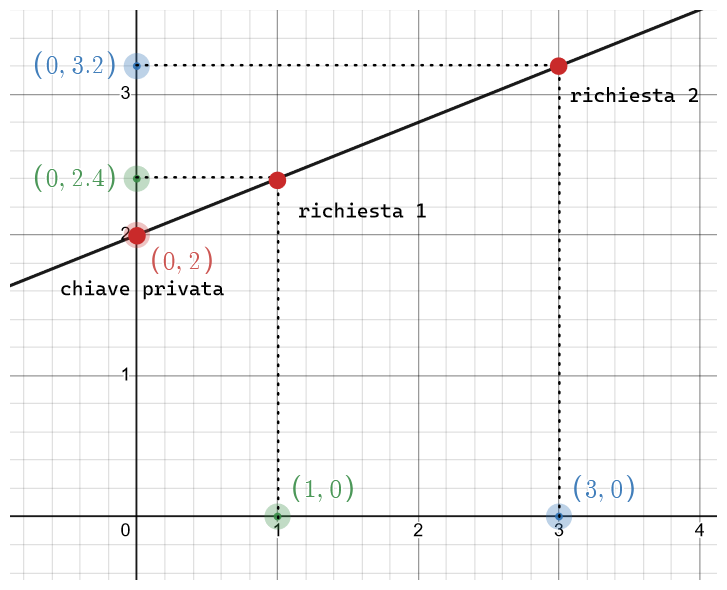
\includegraphics[width=11cm]{./chapters/2.rln-protocol/images/6.a_0_interpolation.png}
    \label{fig:a_0_interpolation}
    \captionsetup{justification=centering}
    \caption{Grafico (SSS) polinomio primo grado}
\end{figure}